\section{Übersicht} 

\subsection{Ausgangslage}
Diese Projekt ist für uns Studenten das erste Projekt mit einem externen Auftraggeberin. Jana Kalbermatter ist eine Designerin, die auch die Fachhochschule Nordwestschweiz besucht hat. Ihre Bachleor-Arbeit möchte sie nun realiseren.

Sie hat eine Art Audio-Guide für Museen designt, welcher sie Dojo nennt. Ihre Arbeit beinhaltete das Design des Gehäse und das dazugehörige Konzept. In ihrem Konzept hat sie die Funktionen des Dojo schon relativ genau definiert, jedoch ist sie offen für neue Ideen. Damit stellt sie die Rahmenbedingungen an das Projekt.

Das Konzept sieht einen Köperschallaktor vor, um die Audio-Files abzuspielen. Eine weitere Eigenheit ist auch der Like Button, mit dem man Ausstellungsstücke " Liken" kann. Diese Likes werden am ende des Museumsbesuch zusammengefasst und in einer nicht genauer definierten Form abgegeben. Ansonsten kann der Dojo das was man von einem Audio-Guide erwarten würde.

Unsere Aufgabe besteht darin in einem ersten Schritt einen funktionierenden Prototypen zu bauen. Dieser soll noch nicht so klein werden, dass er in den Dojo hinein passen kann. Die Integration soll in einem zweiten Schritt erfolgen. Dies dürfen jedoch nur die Teams machen, die einen genügend guten Prototypen haben.

\begin{figure}[H]
\begin{center}
	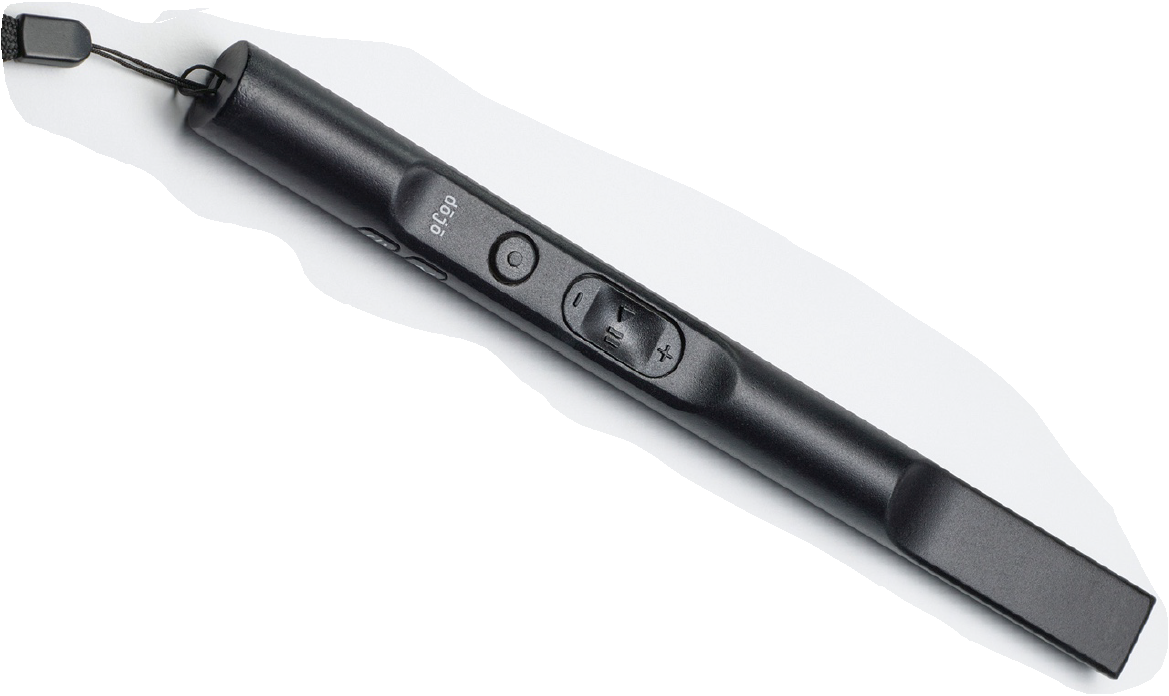
\includegraphics[width=160mm]{data/Ausgangslage_Dojo.png}
	\caption{Konzeptzeichnung des Dojo} %picture caption
	\label{fig:first_layer}
\end{center}
\end{figure}

\pagebreak

\subsection{Projektziele}

\subsection{Lieferobjekte}